% ************************************************************************
\clearpage
\begin{figure}[!t]
\centering
\begin{tabular}{c@{\hspace{0.02\columnwidth}}c@{\hspace{0.02\columnwidth}}c}
\includegraphics[width=0.31\columnwidth]{./fig/p_opf} &% ./fig/compare/opf/p
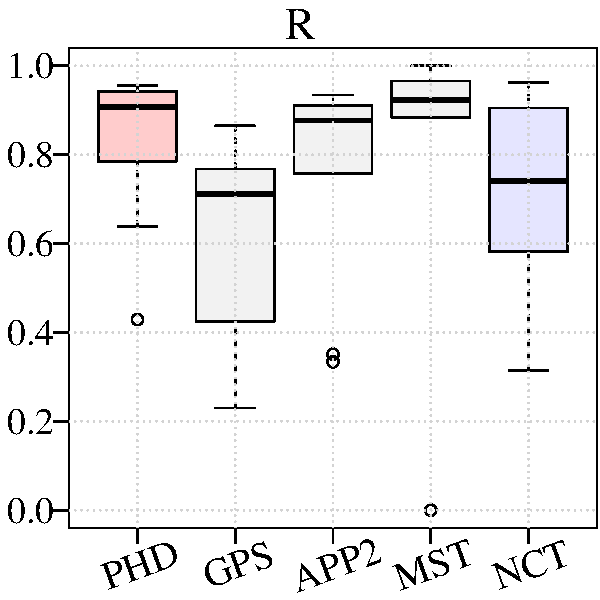
\includegraphics[width=0.31\columnwidth]{./fig/r_opf} &% ./fig/compare/opf/r
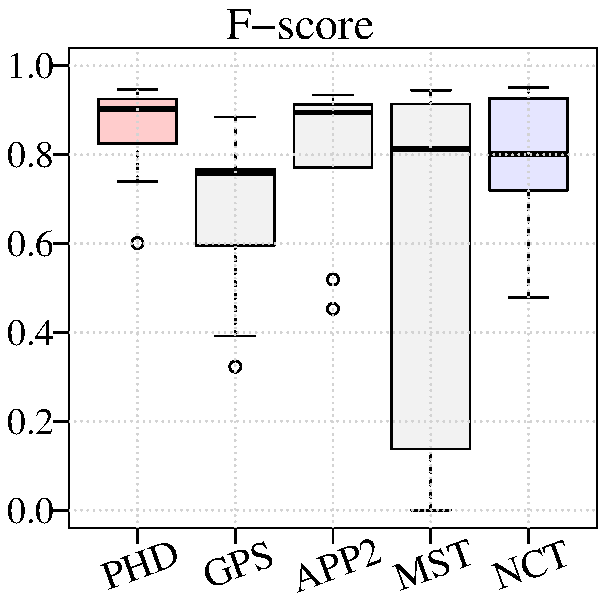
\includegraphics[width=0.31\columnwidth]{./fig/f_opf} \\[1ex]% ./fig/compare/opf/f
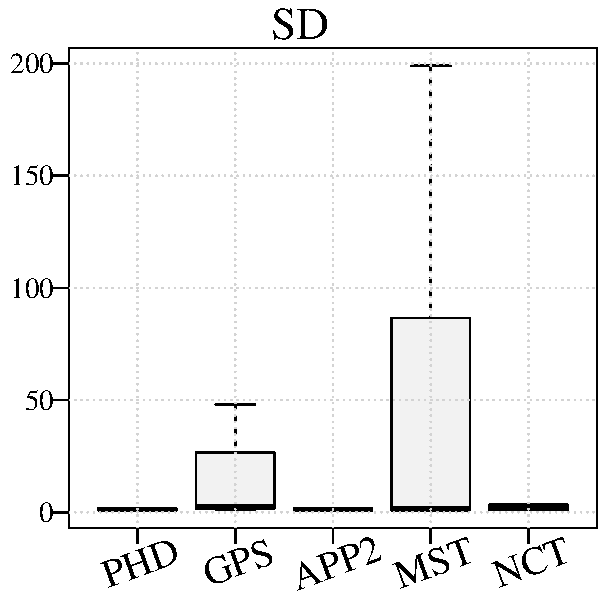
\includegraphics[width=0.31\columnwidth]{./fig/sd_opf} &% ./fig/compare/opf/sd
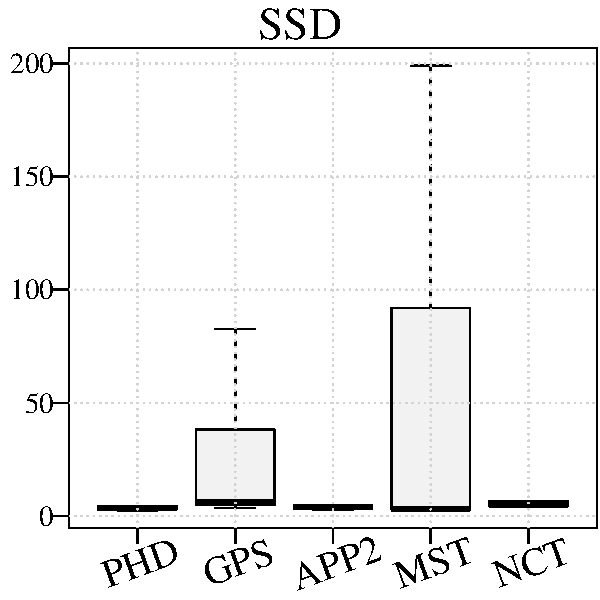
\includegraphics[width=0.31\columnwidth]{./fig/ssd_opf} &% ./fig/compare/opf/ssd
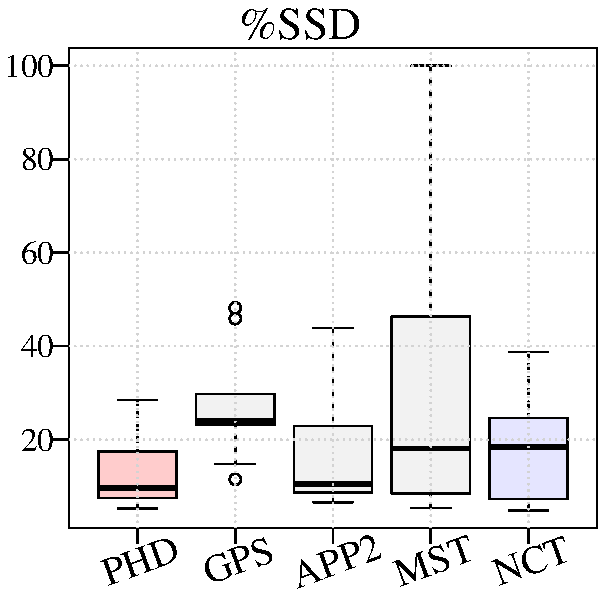
\includegraphics[width=0.31\columnwidth]{./fig/pssd_opf} \\% ./fig/compare/opf/pssd
\end{tabular}
\caption{Performance comparison of our method with several other methods on the OPF data set. For each method and each measure, the plotted box indicates the 25-75 percentile, the horizontal bar indicates the median score, and the whiskers and outliers are drawn using the default settings of R.}
\label{fig:compare-opf}
\end{figure}

% ************************************************************************
\clearpage
\begin{figure}[!t]
\centering
\begin{tabular}{c@{\hspace{0.02\columnwidth}}c@{\hspace{0.02\columnwidth}}c}
\includegraphics[width=0.31\columnwidth]{./fig/p_saria} &% ./fig/compare/saria/p
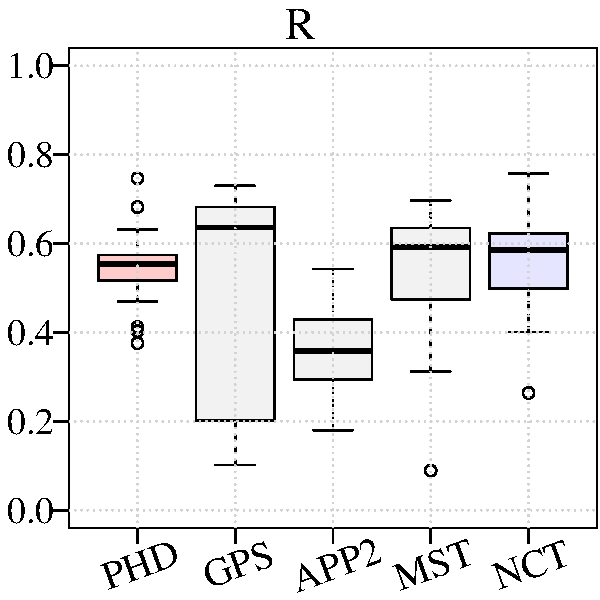
\includegraphics[width=0.31\columnwidth]{./fig/r_saria} &% ./fig/compare/saria/r
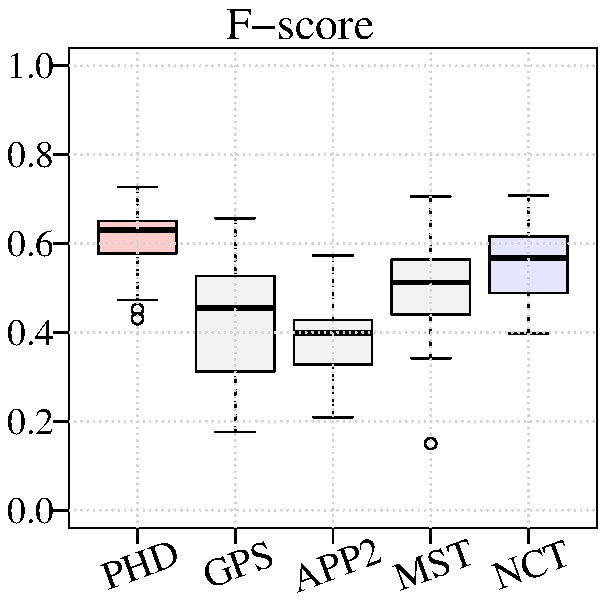
\includegraphics[width=0.31\columnwidth]{./fig/f_saria} \\[1ex]% ./fig/compare/saria/f
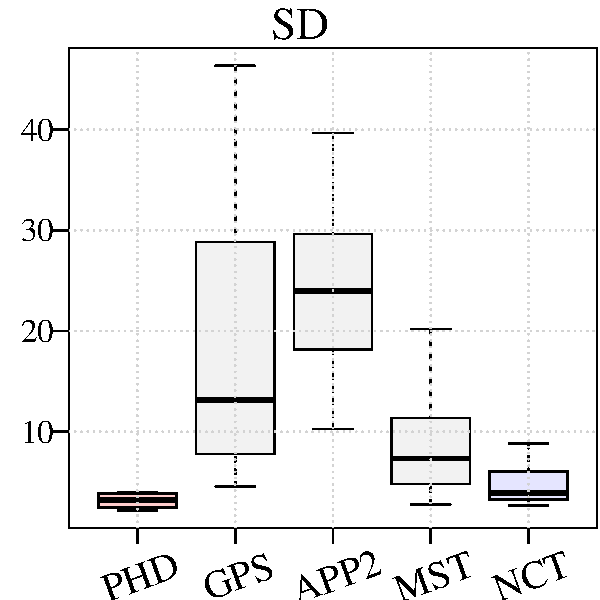
\includegraphics[width=0.31\columnwidth]{./fig/sd_saria} &% ./fig/compare/saria/sd
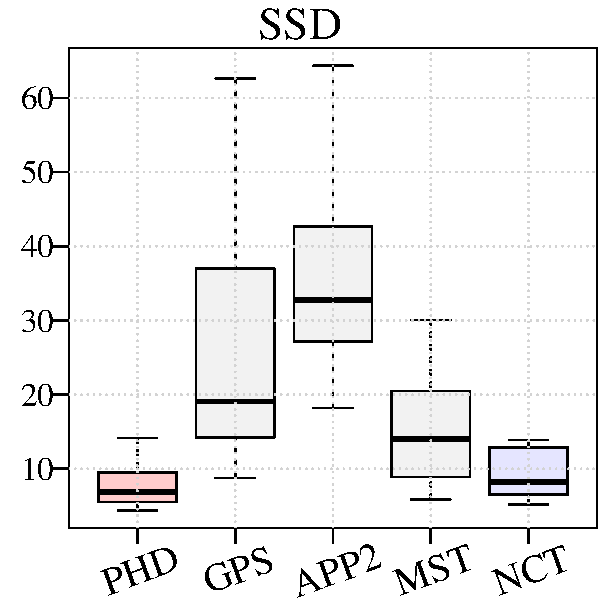
\includegraphics[width=0.31\columnwidth]{./fig/ssd_saria} &% ./fig/compare/saria/ssd
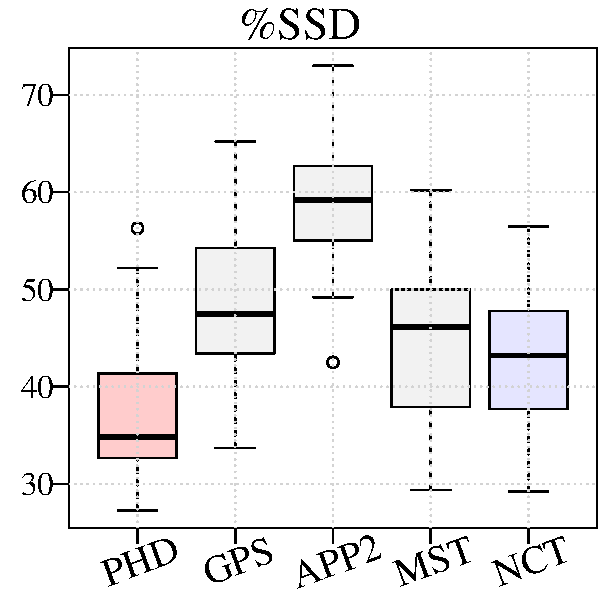
\includegraphics[width=0.31\columnwidth]{./fig/pssd_saria} \\% ./fig/compare/saria/pssd
\end{tabular}
\caption{Performance comparison of our method with several other methods on the HCN data set. For each method and each measure, the plotted box indicates the 25-75 percentile, the horizontal bar indicates the median score, and the whiskers and outliers are drawn using the default settings of R.}
\label{fig:compare-saria}
\end{figure}

% ************************************************************************
\clearpage
\begin{figure}[!t]
\centering
\begin{tabular}{r@{\hspace{0.02\columnwidth}}c@{\hspace{0.02\columnwidth}}c@{\hspace{0.02\columnwidth}}c}
Case: &

\includegraphics[align=c,width=0.15\columnwidth]{./fig/c2.compare/i1_inv} &

\includegraphics[align=c,width=0.15\columnwidth]{./fig/c2.compare/i2_inv} &

\includegraphics[align=c,width=0.15\columnwidth]{./fig/c2.compare/i3_inv}\\
PHD: &
\includegraphics[align=c,width=0.2\columnwidth]{./fig/c2.compare/phd,i1,c0,s0} &
\includegraphics[align=c,width=0.2\columnwidth]{./fig/c2.compare/phd,i2,c0,s0} &
\includegraphics[align=c,width=0.2\columnwidth]{./fig/c2.compare/phd,i3,c0,s0} \\
GPS: &
\includegraphics[align=c,width=0.2\columnwidth]{./fig/c2.compare/gps,i1} &
\includegraphics[align=c,width=0.2\columnwidth]{./fig/c2.compare/gps,i2} &
\includegraphics[align=c,width=0.2\columnwidth]{./fig/c2.compare/gps,i3} \\
APP2: &
\includegraphics[align=c,width=0.2\columnwidth]{./fig/c2.compare/app2,i1} &
\includegraphics[align=c,width=0.2\columnwidth]{./fig/c2.compare/app2,i2} &
\includegraphics[align=c,width=0.2\columnwidth]{./fig/c2.compare/app2,i3} \\
MST: &
\includegraphics[align=c,width=0.2\columnwidth]{./fig/c2.compare/mst,i1} &
\includegraphics[align=c,width=0.2\columnwidth]{./fig/c2.compare/mst,i2} &
\includegraphics[align=c,width=0.2\columnwidth]{./fig/c2.compare/mst,i3} \\
\end{tabular}
\caption{Ability of the tested methods to separate two fibers of similar intensity and scale running closely in parallel. The examples show cases with gradually increasing distance between the fibers: overlap (left column), just separated (middle column), and clearly separated (right column). The tracing results of PHD, GPS, APP2, MST are overlaid (with slight offset) in red color.}
\label{fig:phd-advantage-2}
\end{figure}

% ************************************************************************
\clearpage
\begin{figure}[!t]
\centering
\begin{tabular}{c@{\hspace{0.02\columnwidth}}c@{\hspace{0.02\columnwidth}}c@{\hspace{0.02\columnwidth}}c}
%\multicolumn{4}{c}{\includegraphics[align=c,width=0.2\columnwidth]{./fig/test2d.compare/i}}\\
Case: &

\includegraphics[align=c,width=0.15\columnwidth]{./fig/c3.compare/i1_inv} &

\includegraphics[align=c,width=0.15\columnwidth]{./fig/c3.compare/i2_inv} &

\includegraphics[align=c,width=0.15\columnwidth]{./fig/c3.compare/i3_inv}\\
PHD: &
\includegraphics[align=c,width=0.2\columnwidth]{./fig/c3.compare/phd,i1,c0,s0} &
\includegraphics[align=c,width=0.2\columnwidth]{./fig/c3.compare/phd,i2,c0,s0} &
\includegraphics[align=c,width=0.2\columnwidth]{./fig/c3.compare/phd,i3,c0,s0} \\
GPS: &
\includegraphics[align=c,width=0.2\columnwidth]{./fig/c3.compare/gps,i1} &
\includegraphics[align=c,width=0.2\columnwidth]{./fig/c3.compare/gps,i2} &
\includegraphics[align=c,width=0.2\columnwidth]{./fig/c3.compare/gps,i3} \\
APP2: &
\includegraphics[align=c,width=0.2\columnwidth]{./fig/c3.compare/app2,i1} &
\includegraphics[align=c,width=0.2\columnwidth]{./fig/c3.compare/app2,i2} &
\includegraphics[align=c,width=0.2\columnwidth]{./fig/c3.compare/app2,i3} \\
MST: &
\includegraphics[align=c,width=0.2\columnwidth]{./fig/c3.compare/mst,i1} &
\includegraphics[align=c,width=0.2\columnwidth]{./fig/c3.compare/mst,i2} &
\includegraphics[align=c,width=0.2\columnwidth]{./fig/c3.compare/mst,i3} \\
\end{tabular}
\caption{Ability of the tested methods to separate three fibers with different intensity and scale running closely in parallel. The examples show cases with gradually increasing distance between the fibers: overlap (left column), just separated (middle column), and clearly separated (right column). The tracing results of PHD, GPS, APP2, MST are overlaid (with slight offset) in red color.}
\label{fig:phd-advantage-3}
\end{figure}

% ************************************************************************
\end{document}
% ************************************************************************